\chapter{Background}

% TODO: Maybe something about assumed knowledge

% TODO: Maybe a notation section
Notation: we write $1$ for the neutral element of a group.

\section{Coxeter Groups}

\begin{definition}
    A \textit{Coxeter system} $(W,S)$ is a group $W$ and a finite subset $S = \{s_1, ..., s_n\} \subset W$ under the following conditions. For any $s,t \in S$, $(st)^{m_{st}} = 1$ where $m_{st} \in \Z_{>0}\cup\{\infty\}$ such that  $m_{st} = 1$ if $s = t$, and $m_{st} = m_{ts} \in \{2,3,...\} \cup \{\infty\}$ if $s \neq t$. In other words, $W = \angl{s \in S \mathrel{|} (st)^{m_{st}} = 1}$ with generator $S$. We call $W$ a \textit{Coxeter group}.
\end{definition}

The value $m_{st} = \infty$ indicates there are no relations of the form $(st)^{m} = 1$ for any $m \in \Z_{>0}$. We often call relations of the form $s^2 = 1$ \textit{quadratic relations}. The quadratic relations on the generators of the Coxeter group imply that $s^{-1} = s$ and $(st)^{-1} = t^{-1} s^{-1} = ts$. Moreover, if $s \neq t$ and $m_{st} < \infty$, then we can use the quadratic relations to write $(st)^{m_{st}} = 1$ equivalently as
\[
    \underbrace{sts...}_{m_{st}} = \underbrace{tst...}_{m_{st}},
\]
which we call \textit{braid relations}.
% TODO: Add reference to why they are called braid relations
Coxeter systems are closely related to reflections, so we often call elements of $S$ \textit{simple reflections}, and elements in $W$ that are conjugates to elements in S \textit{reflections}.
% TODO: Add reference to why they are reflections (ch2, or of it is added to this paper)

\begin{example}\label{example-CG}
    The permutation group of $n$ elements $S_n$ is a Coxeter group generated by the set of transpositions $S = \{(i,i+1) \in S_n : 1 \leq i \leq n-1\}$. Let $s_i := (i,i+1)$. We know from algebra that $S$ generates $S_n$, so let us check the relations.
    \begin{itemize}
        \item For any $i$, $s_i^2 = (i,i+1)(i,i+1) = 1$.
        \item For $i > j+1$, the transpositions $(i,i+1)$ and $(j,j+1)$ are disjoint so $(s_i s_j)^2 = (i,i+1)(j,j+1)(i,i+1)(j,j+1) = 1$.
        \item For $i = j+1$, $(s_i s_j)^3 = ((i,i+1)(j,j+1))^3 = (i,i+1,i+2)^3 = 1$.
    \end{itemize}
    These are sometimes called the Coxeter system of type $A_{n-1}$, for $n \geq 2$.

    An easy case is the Coxeter group $W \simeq S_3$ with generators $S = \{s,t\}$ where $s,t$ correspond to transpositions $(12)$ and $(23)$ respectively. By the quadratic and braid relations, we find that the elements of $W$ are exactly $1,s,t,st,ts,sts=tst$. We will frequently revisit this example. % REVIEW: Rewrite this last sentence after I have used it more

    % TODO: Should I add more details?
\end{example}

\begin{definition}
    Let $w \in W$. As $S$ generates $W$, we can write $w = s_1 s_2 ... s_k$ for some $s_1,...,s_k \in S$. We say the sequence $(s_1, ..., s_k)$ is an \textit{expression} for $w$ of \textit{length} $k$. Given the relations in the definition, $w \in W$ is not uniquely expressed as such a sequence, so we write $\ul{w}$ to denote a choice of expression $(s_1, ..., s_k)$ for $w$.
\end{definition}

\begin{definition}
    Let $w \in W$. For any expression $\underline{w} = (s_1, ..., s_k)$, we say the \textit{length of $\underline{w}$} is $k$, and write $\ell(\ul{w}) = k$. The \textit{length of $w$}, written $\ell(w)$ is the smallest integer $k$ such that $w$ admits an expression of length $k$. We say an expression $\ul{w}$ is \textit{reduced} if $\ell(\ul{w}) = \ell(w)$.
\end{definition}

Note that $\ell(w) = 0$ if and only if $w = 1$.

The following are useful results regarding reduced expressions. % TODO: reword this

\begin{theorem}[Exchange condition]
    Let $\underline{w} = (s_1, ..., s_k)$ be a reduced expression for $w \in W$, and let $t \in S$. If $\ell(wt) < \ell(w)$, then there exists an integer $i \in \{1,2,...,k\}$ such that $wt = s_1 ... \hat{s_i} ... s_k$, i.e. with $s_i$ omitted.
\end{theorem}

% TODO: Proof?
% TODO: Example?

\begin{corollary}[Deletion Condition]
    Let $\underline{w} = (s_1, ..., s_k)$ be an expression for $w \in W$ where $\ell(w) < k$, i.e. not a reduced expression. Then there exists some $i < j$ such that $w = s_1 ... \hat{s_i} ... \hat{s_j} ... s_k$.
\end{corollary}

In other words, if an expression is not reduced, two elements in the expression may be cancelled to result in a shorter expression.

% TODO: Proof?
% TODO: Example?

\begin{theorem}[Matsumoto, 1964]\label{thm-matsumoto}
    Any two reduced expressions for $w \in W$ are related by braid relations.
\end{theorem}

% TODO: Put a proof, or reference to one

We can also define a partial order on $W$.
% TODO: What is this used for?

\begin{definition}[Bruhat Order]
    Let $T$ be the set of elements of $W$ that are conjugate to elements in $S$. Define a partial order $\leq$ on $W$ such that for $x,y \in W$, $x \leq y$ if and only if there exists a chain $x=x_0,x_1,...,x_m=y$ of elements in $W$ such that $\ell(x_i) < \ell(x_{i+1})$ and $x_i^{-1} x_{i+1} \in T$ for each $i = 0,1,...,m-1$.
\end{definition}

That is $x_{i+1}$ is $x_i$ multiplied on the right with a conjugate of an element in $S$ such that its length is longer than $x_i$. Note that we can equivalently multiply on the left because for any $t \in T$ we can write $xt = (xtx^{-1})x$ where $xtx^{-1} \in T$.

% TODO: Explain why we need T

Equivalently let $y = s_1 ... s_k$ be a reduced expression, and we can define $x \leq y$ to be if and only if there exists a reduced expression $x = s_{i_1} ... s_{i_\ell}$ such that $1 \leq i_1 < ... < i_\ell \leq k$. In other words, $x$ is $y$ after removing some terms from a reduced expression (we say $x$ is a \textit{subexpression} of $y$).

% TODO: Why is it equivalent? (Exercise 1.64)

\begin{example}
    The Hasse diagram for the Bruhat order on $S_3$ is as follows (using the labelling of elements from Example \ref{example-CG}).
    \begin{center}
        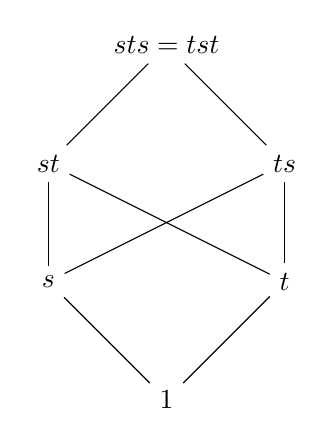
\begin{tikzpicture}
            \node (1) at (0,0) {$1$};
            \node (s) at (-1.5,1.5) {$s$};
            \node (t) at (1.5,1.5) {$t$};
            \node (st) at (-1.5,3) {$st$};
            \node (ts) at (1.5,3) {$ts$};
            \node (sts) at (0,4.5) {$sts=tst$};

            \draw (1)--(s);
            \draw (1)--(t);
            \draw (s)--(st);
            \draw (t)--(st);
            \draw (s)--(ts);
            \draw (t)--(ts);
            \draw (st)--(sts);
            \draw (ts)--(sts);
        \end{tikzpicture}
    \end{center}
\end{example}


\begin{definition}
    Given a Coxeter system $(W,S)$, define a representation $V$ of $W$ as follows. Let $V$ be a vector space over $\R$ generated by the basis $\{\alpha_s : s \in S\}$. Equip $V$ with a symmetric bilinear form $(-,-)$ defined by
    \[
        (\alpha_s, \alpha_t) = - \cos \frac{\pi}{m_{st}}.
    \]
    If $m_{st} = \infty$ we define $\pi/m_{st} = 0$. Define the $W$-action on $V$ such that for $s \in S$ and $v \in V$,
    \[
        s \cdot v = v - 2(v,\alpha_s) \alpha_s.
    \]
    We call this the \textit{geometric representation} of the Coxeter system.
\end{definition}

This is defined for both finite and infinite Coxeter groups.

% Some geometric intuition, vectors are vectors, and action of $s \in S$ is reflection across the hyperplane with normal as the vector corresponding to $s$

\begin{proposition}
    For any Coxeter system, the geometric representation is faithful.
\end{proposition}

% TODO: Proof?

In this paper, we will work with this representation of the Coxeter group.
% Briefly discuss other representations (eg. Kac-moody representation)


\section{Hecke Algebra}

% TODO: Introduction/motivation

Let $\Z[v, v^{-1}]$ be the set of integer Laurent polynomials, for an indeterminate $v$.

\begin{definition}
    The \textit{Hecke algebra} $\cH$ for a Coxeter system $(W,S)$ is the unital associative algebra over $\Z[v,v^{-1}]$ generated by $\{\delta_s : s \in S\}$ with the following relations.
    \begin{itemize}
        \item $\delta_s^2 = (v^{-1} - v)\delta_s + 1$, for any $s \in S$.
        \item $\underbrace{\delta_s \delta_t \delta_s...}_{m_{st}} = \underbrace{\delta_t \delta_s \delta_t...}_{m_{st}}$, for any $s,t \in S$ where $m_{st} < \infty$.
    \end{itemize}
\end{definition}

Recall that an algebra over a commutative ring $R$ is an $R$-module with an $R$-bilinear multiplication operation. A unital associative algebra over $R$ is then an algebra over $R$ for which multiplication is associative and has a multiplicative identity.

Similarly to Coxeter groups, we call the first relations \textit{quadratic relations} and the second \textit{braid relations}.

% TODO: Why is the quadratic relation is the way it is

Note that the quadratic relation is equivalent to $(\delta_s - v^{-1})(\delta_s + v) = 0$.

% TODO: Why? Why is this important?


% REVIEW: Add more on how it relates to coxeter groups
% \begin{remark}
%     If $A$ is a commutative ring, then a ring homomorphism $\phi: \Z[v ,v^{-1}] \to A$ gives $A$ the structure of a $\Z[v,v^{-1}]$-algebra.
%     % (TODO: so that the action of $x \in \Z[v,v^{-1}]$ on $a \in A$ is $x \cdot a = \phi(x) a$??).
%     With this we can form the specialisation $\cH_\phi := A \otimes_{\Z[v,v^{-1}]} \cH$ of $\cH$.
%     % (Look more into what specialisation is and does.)
%     Note that this specialisation is uniquely determined by the ring $A$ and the invertible element $\phi(v) \in A^\times$.
%     In particular if $A = \Z$ and $\phi(v) = 1$, the specialisation of $\cH$ is isomorphic to the group algebra $\Z[W]$ (mapping $\delta_s$ to $s \in S$). Because of this, the Hecke algebra is a \textit{deformation} of the group algebra of $W$. Also notice that in the specialisation $v \mapsto 1$, the quadratic relation of the Hecke algebra becomes the quadratic relation of the Coxeter group.
%     % TODO: What does this say about Hecke algebra and coxeter groups?
% \end{remark}

For $w \in W$ with reduced expression $w = s_1 s_2 ... s_k$, define the element $\delta_w = \delta_{s_1}  \delta_{s_2} ... \delta_{s_k}$ of $\cH$. Since $\cH$ has braid relations identical to $W$, Matsumoto's theorem (Theorem \ref{thm-matsumoto}) implies that this is independent of the choice of reduced expression. Note that we set $\delta_1 = 1$


\begin{theorem}
    The Hecke algebra is a free $\Z[v,v^{-1}]$-module with basis $\{\delta_w : w \in W\}$.
\end{theorem}

\begin{definition}
    We call $\{\delta_w : w \in W\}$ the \textit{standard basis} of $\cH$.
\end{definition}


\begin{proposition}
    The following multiplication formulae hold in $\cH$. For $w \in W$ and $s \in S$,
    \[
        \delta_w \delta_s =
        \begin{cases}
            \delta_{ws}                        & \text{if } ws > w, \\
            (v^{-1} - v)\delta_w + \delta_{ws} & \text{if } ws < w, \\
        \end{cases}
    \]
    and
    \[
        \delta_s \delta_w =
        \begin{cases}
            \delta_{sw}                        & \text{if } ws > w, \\
            (v^{-1} - v)\delta_w + \delta_{sw} & \text{if } ws < w. \\
        \end{cases}
    \]
\end{proposition}

\begin{proposition}
    For any simple reflection $s \in S$,
    \[
        \delta_s^{-1} = \delta_s + (v - v^{-1}).
    \]
\end{proposition}
This follows from the quadratic relation in $\cH$.

\begin{proposition}
    Since the generators $\{\delta_s : s \in S\}$ of $\cH$ are invertible, $\delta_w$ is invertible for every $w \in W$. Moreover,
    \[
        \delta_{w^{-1}}^{-1} = \delta_w + \sum_{x < w} a_x \delta_x
    \]
    for some $a_x \in \Z[v,v^{-1}]$.
\end{proposition}

% \grey{Kazhdan-Lusztig Basis}

There is another basis known as the Kazhdan-Lusztig basis.

\begin{definition}
    The \textit{Kazhdan-Lusztig involution} or \textit{bar involution} is a $\Z$-linear involution $\cH \to \cH, h \mapsto \ol{h}$ defined on generators $\ol{v} = v^{-1}$ and $\ol{\delta_s} = \delta_s^{-1}$ for $s \in S$, such that it distributes across products as a ring automorphism.
\end{definition}

% REVIEW: CHeck if we need: \ol{\deta_w} = \delta_{w^{-1}}^{-1}

\begin{definition}
    The \textit{Kazhdan-Lusztig basis} for $\cH$ is the set $\{b_w : w \in W\} \subseteq \cH$ such that for any $w \in W$,
    \begin{itemize}
        \item $b_x$ is self-dual, i.e. $\ol{b_x} = b_x$, and
        \item $b_x$ has the form
              \[
                  b_x = \delta_x + \sum_{y<x} h_{y,x} \delta_y
              \]
              for some $h_{y,x} \in v\Z[v]$, where $<$ is the Bruhat order.
    \end{itemize}
    The coefficients $h_{y,x} \in v\Z[v]$ are called \textit{Kazhdan-Lusztig polynomials}.
\end{definition}

Additionally, we set $h_{x,x} = 1$ and $h_{y,x} = 0$ if $y \not\leq x$ in the Bruhat order. The second condition is sometimes called the \textit{degree bound} condition.

\begin{lemma}
    The Kazhdan-Lusztig basis is unique.
\end{lemma}

Furthermore, the corresponding Kazhdan-Lusztig basis element for $s \in S$ is $b_s = \delta_s + v$.

% \grey{Standard Form}
% REVIEW: Do we need this? When is this used later?
% TODO: Why is this important? When do we see this later?

\begin{definition}
    The \textit{Kazhdan-Lusztig anti-involution} $\omega: \cH \to \cH$ is an involution defined similarly to the Kazhdan-Lusztig involution, but distributes across products as a ring \textit{anti}-automorphism. That is for $a,b \in \cH$, $\omega(ab) = \omega(b) \omega(a)$.
\end{definition}

\begin{definition}
    The \textit{standard trace} $\epsilon: \cH \to \Z[v,v^{-1}]$ is a $\Z[v,v^{-1}]$-linear map which extracts the coefficient of $\delta_{id}$ for elements written in the standard basis.
\end{definition}

\begin{definition}
    The \textit{standard form} $(-,-): \cH\times\cH \to \Z[v,v^{-1}]$ is a sesquilinear form (with respect to either involution restricted to $\Z[v,v^{-1}]$) such that $(a,b) := \epsilon(\omega(a)b)$ for $a,b \in \cH$.
\end{definition}
% TODO: Motivation for this definition
Here, sesquilinear means that the form is linear in the second variable and in the first variable, $(fa,b) = \ol{f} (a,b)$ for $a,b \in \cH$ and $f \in \Z[v,v^{-1}]$. Note the restricted involution inverts each $v$ extending linearly to $\Z[v,v^{-1}]$. The bar involution and anti-involution restricted to $\Z[v,v^{-1}]$ are the same, as this ring is commutative.

% What do we need?
% Cor 3.18?
% Lemma 3.19? For calculating standard form on self dual elements

\begin{theorem}
    The Kazhdan-Lusztig basis is asymptotically orthonormal. That is for $x,y \in W$,
    \[
        (b_x, b_y) =
        \begin{cases}
            1 + v\Z[v] & \text{if }x = y,  \\
            v\Z[v]     & \text{otherwise.}
        \end{cases}
    \]
\end{theorem}

% Comment on the naming. Normal when v=0.


% \grey{Construction of Kazhdan-Lusztig basis}
% REVIEW: Do we need this?
% TODO: Will probably need introduction of coxter complexes to have a diagram to do examples

% \grey{Category Theory}
% \grey{(To introduce category theory concepts when we need them)}
% TODO: introduce category theory concepts when we need them


\section{Soergel Bimodules}

% TODO: A brief intro into what they are, and what we need to define them. (Some motivation for gradings, etc.)

\begin{definition}
    A \textit{$\Z$-graded ring} $R$ is a ring with a decomposition
    \[
        R = \bigoplus_{i \in \Z} R^i
    \]
    into a direct sum of additive subgroups $R_i \subseteq R$ such that $R^i R^j \subseteq R^{i+j}$.
\end{definition}

Gradings are defined in this way to generalise a notion of 'degree', where the degree of a product is the sum of their degrees. % TODO: This is intuition for definition, but do we ever use this?
This definition can naturally be extended to $\Z$-graded modules over some a $\Z$-graded ring.

\begin{definition}
    Let $R$ be a $\Z$-graded ring. A \textit{$\Z$-graded $R$-module} $M$ is a module over $R$ with a decomposition
    \[
        M = \bigoplus_{i \in \Z} M^i
    \]
    into a direct sum of additive subgroups $M^i \subseteq M$ such that $R^i M^j \subseteq M^{i+j}$. We call the $M^i$ \textit{graded pieces} of $M$, and the elements of $M^i$ \textit{homogeneous of degree $i$}.
\end{definition}

For the remainder of this paper we will only be working with $\Z$-graded objects, so we just say \textit{graded}.

\begin{example}
    For any ring $R$, the \textit{trivial grading} of $R$ is the decomposition where $R^0 = R$ and $R^i = 0$ for all $i \neq 0$.
\end{example}

\begin{example}
    Let $F$ be a field with the trivial grading. The vector space of real polynomials (in one or several variables) over $F$ has a natural grading where the $n$-graded piece is the subspace generated by degree $n$ monomials. For example, the $\R$-vector space $\R[x]$ has a decomposition
    \[
        \R[x] = V^0 \oplus V^1 \oplus V^2 \oplus \dots
    \]
    where $V^i$ is the subspace spanned by $\{x^i\}$. This example is a $\Z$-grading where the $n$-graded piece is $0$ for $n < 0$.
\end{example}

Gradings for other algebraic objects, such as algebras and bimodules, can be similarly defined. The following definitions are for general graded objects.

\begin{definition}
    Let $M$ and $N$ be graded objects. For $i \in \Z$, define $M(i)$ to be the graded object with graded pieces $M(i)^j \coloneqq M^{i+j}$. We say this is obtained by a \textit{shift in grading} of $M$.
\end{definition}

If we visualise the graded pieces horizontally in ascending order of degree, the grading of $M(i)$ is the grading of $M$ shifted to the left by $i$ places. Particularly, if $x \in M^n$ is homogeneous of degree $n$ in $M$, then it is homogeneous of degree $n - i$ in $M(i)$.
\begin{center}
    \begin{tabular}{ |r||c|c|c|c|c| }
        \hline
        \textbf{Degree} & $-2$       & $-1$       & $0$      & $1$       & $2$       \\ \hline
        $M$             & $M^{-2}$   & $M^{-1}$   & $M^0$    & $M^1$     & $M^2$     \\ \hline
        $M(1)$          & $M^{-1}$   & $M^0$      & $M^1$    & $M^2$     & $M^3$     \\ \hline
        $M(2)$          & $M^0$      & $M^1$      & $M^2$    & $M^3$     & $M^4$     \\ \hline
        $M(-1)$         & $M^{-3}$   & $M^{-2}$   & $M^{-1}$ & $M^0$     & $M^1$     \\ \hline
        $M(i)$          & $M^{-2+i}$ & $M^{-1+i}$ & $M^{i}$  & $M^{1+i}$ & $M^{2+i}$ \\ \hline
    \end{tabular}
\end{center}

\begin{definition}
    Let $M$ and $N$ be graded objects. A morphism $f: M \to N$ is \textit{homogeneous of degree $k$} if $f(M^i) \subseteq N^{i+k}$ for all $i \in \Z$. Typically we assume morphisms between graded objects are homogeneous of degree $0$, and call them \textit{graded morphisms}. A \textit{graded isomorphism} is a graded morphism with a graded (two-sided) inverse. We say that $M$ and $N$ are \textit{isomorphic up to shift} if there is a graded isomorphism $M \simeq N(i)$ for some $i \in \Z$. The \textit{graded morphism space} (or \textit{graded Hom space}) between $M$ and $N$ is
    \[
        \Hom^\bullet(M,N) \coloneqq \bigoplus_{i \in \Z} \Hom(M,N(i)).
    \]
\end{definition}

Notice for any morphism $M \to N$ of degree $k$, there is a morphism $M \to N(k)$ of degree $0$ that contains the same information.
% We don't care too much about degree 0 morphisms from $M(-k) \to N$ (that have the same information), because want the domain to be fixed. Probably similar reason that the graded hom space only shifts the codomain.

\begin{definition}
    Let $M$ be a graded object in an additive category (i.e. direct sums are defined on $M$), and let $p = \sum_i p_i v^i \in \Z_{\geq 0}[v^{\pm 1}]$ be a Laurent polynomial with positive integer coefficients. Define
    \[
        M^{\oplus p} \coloneqq \bigoplus_{i \in \Z} M(i)^{\oplus p_i}
    \]
    where $M^{\oplus k} \coloneqq \bigoplus_{j=1}^k M$ for $k \in \Z_{\geq 0}$.
\end{definition}



\begin{definition}
    Let $R$ be a graded ring and $M$ a graded $R$-module. A \textit{graded submodule} of $M$ is a submodule $N \subseteq M$ with the induced grading $N^i = N \cap M^i$ for all $i \in \Z$. A \textit{graded direct summand} of $M$ is a graded module $N$ such that $M \simeq N \oplus N'$ as graded modules for some graded submodule $N' \subseteq M$.
    % Might not need this: "A graded submodule $N \subseteq M$ is a graded direct summand iff it is a direct summand of ungraded modules. (Need to show that if $M \simeq N \oplus N'$ as ungraded direct sum, then $N'$ turns out to be a graded submodule.)"
    We say that $M$ is \textit{graded free} if it has an $R$-basis of homogeneous elements of $M$. If this basis is finite, then there is a unique $p \in \Z_{\geq 0}[v^{\pm 1}]$ such that $M \simeq R^{\oplus p}$, and we call $p$ the \textit{graded rank} of $M$.
\end{definition}


For our purposes, fix a Coxeter system $(W,S)$ and consider it's geometric representation $V$. Let $R = \op{Sym}(V) \simeq \R[\alpha_s : s \in S]$ be the symmetric algebra of $V$, which we will think of as the real polynomial ring generated, as a ring, by the basis of $V$. We can think of $R$ as a graded algebra\footnote{A graded module that is also a graded ring.}, such that $V \subseteq R$ is homogeneous of degree $2$, i.e. $\deg \alpha_s = 2$ and the `monomials' that are products of $i$ basis elements are degree $2i$.
% Why are all the gradings doubled?
% Maybe note that we take the trivial grading for $\R$.

There is a natural action of $W$ on $R$, induced by its action on $V$, that for any $w \in W$,
\[
    w \cdot \prod_{s \in S} \alpha_s^{k_s} = \prod_{s \in S} (w \cdot \alpha_s)^{k_s}
\]
where $k_s \in \Z_{\geq 0}$, extending linearly to $R$.

% What are soergel bimodules? How are they related to this?
% What do we need to define to get there?




